\pdfoutput=1
\documentclass[a4paper,onecolumn,unpublished]{quantumarticle}
\pdfoutput=1

\usepackage[utf8]{inputenc}
\usepackage[T1]{fontenc}
\usepackage{amsmath,amssymb,amsfonts,amsthm,mathtools}
\usepackage{bm}
\usepackage{booktabs}
\usepackage{graphicx}
\usepackage{xcolor}
\usepackage[section]{placeins}
\usepackage{hyperref}

\newcommand{\Prob}{\mathbb{P}}
\newcommand{\E}{\mathbb{E}}
\newcommand{\F}{\mathcal{F}}
\newcommand{\G}{\mathcal{G}}
\newcommand{\Hfil}{\mathcal{H}}
\newcommand{\R}{\mathbb{R}}
\newcommand{\ind}{\mathbb{I}}
\providecommand{\ket}[1]{\lvert #1 \rangle}
\providecommand{\bra}[1]{\langle #1 \rvert}
\providecommand{\mel}[3]{\langle #1 \vert #2 \vert #3 \rangle}
\newcommand{\Fdisc}{\mathcal{F}_{\mathrm{disc}}}
\newcommand{\Bdisc}{B_{\mathrm{disc}}}
\newcommand{\Bconf}{B_{\mathrm{conf}}}
\newcommand{\Ndisc}{N_{\mathrm{disc}}}
\newcommand{\Nconf}{N_{\mathrm{conf}}}
\newcommand{\adisc}{\alpha_{\mathrm{disc}}}
\newcommand{\aconf}{\alpha_{\mathrm{conf}}}
\newcommand{\aup}{\alpha_{\mathrm{conf,up}}}
\newcommand{\alow}{\alpha_{\mathrm{conf,low}}}
\newcommand{\epsbest}{\epsilon_{\mathrm{best}}}
\newcommand{\ddrift}{\delta_{\mathrm{drift}}}
\newcommand{\Kmax}{K_{\max}}
\renewcommand{\th}{\bm{\theta}}
\newcommand{\thhat}{\widehat{\bm{\theta}}}

\begin{document}

\title{Tripura: Discover--Freeze--Certify for Anytime-Valid Certification of Finite-Shot Variational Quantum Optimization}

\author{Nimma Sudhamsh Reddy}
\affiliation{Department of Electronics and Communication Engineering, Amrita School of Engineering, Coimbatore, Amrita Vishwa Vidyapeetham, India}
\email{cb.en.u4cce24136@cb.students.amrita.edu}

\maketitle

\begin{abstract}
\noindent In finite-shot variational quantum optimization, the parameter vector that looks best on noisy data is usually also the one that was helped most by that noise. Using the same measurements both to pick this vector and to certify that its true objective meets a target is therefore unsafe: the estimate is biased downward (the winner's curse), and stopping early when the data look good makes it worse. We present Tripura, a three-phase protocol (discover, freeze, certify). Phase~A searches adaptively and spends shots on the leading candidates using confidence sequences. Phase~B freezes one candidate without using any shots. Phase~C tests that candidate on a fresh measurement stream with an anytime-valid sequential test, whose false-certification probability is at most $\aconf$ whatever happened in Phase~A. We quantify the selection bias, prove the guarantees, and test the protocol on 500 three-regular QAOA MaxCut instances ($n \in \{12, 14\}$, $p = 2$) using exact statevector simulation with finite-shot sampling. Under a matched 2,560-shot discovery budget, the deployable version (Mode~U) used $3331.5 \pm 89.2$ shots in total, $49.9\%$ fewer than a fixed 4096-shot confirmation baseline, with $0/500$ false certifications. We also study common random numbers (CRN), which are available only in simulation, and show where they keep the Phase~A guarantees and where they break them. Part of the saving comes from sequential stopping alone, and we report that split. All results are from simulation; hardware runs and larger instances are left for future work.
\end{abstract}

\section{Introduction}
\label{sec:intro}

Variational quantum algorithms such as the Quantum Approximate Optimization Algorithm (QAOA) \cite{farhi2014} and the Variational Quantum Eigensolver (VQE) \cite{cerezo2021} train a parameterized circuit with a classical optimizer. Every objective evaluation comes from a finite number of measurement shots, so it is a noisy estimate. At the end of a run one usually wants a statement of the form ``the selected parameters $\thhat$ achieve risk $\mu(\thhat) \le \tau$, with error probability at most $\aconf$.''

Obtaining such a statement is harder than it looks. The optimizer visits many parameter vectors and keeps the one with the best empirical value. That value is optimistic, because selecting a minimum of noisy estimates favours estimates that happened to be too low. If the same data are then used for certification, the stated error probability no longer holds. Stopping the measurements as soon as the data look convincing adds a second source of inflation \cite{dwork2015,ramdas2023}.

Existing shot-frugal optimizers such as Rosalin \cite{arrasmith2020}, iCANS \cite{kuebler2020} and gCANS \cite{gu2021} reduce the measurement cost of the search, but they are not designed to give a post-selection certificate. Sequential statistics offers the missing tools: time-uniform empirical-Bernstein confidence sequences \cite{howard2021}, betting-based confidence sequences \cite{waudby2024}, and best-arm racing rules such as LUCB \cite{kalyanakrishnan2012}. These are usually stated for fixed candidate pools with independent streams, whereas an optimizer such as COBYLA \cite{powell1994} creates candidates adaptively from earlier noisy outcomes.

\paragraph*{Contributions.}
This paper combines these existing tools into one protocol, which we call Tripura\footnote{Tripura is Sanskrit for ``three cities'' or ``three realms''. In Indian philosophy it is also linked to the three states of consciousness (waking, dreaming, deep sleep). We use the name only as a mnemonic for the three phases of the protocol.} for variational optimization and analyses the points where adaptivity causes trouble.
\begin{enumerate}
  \item \textbf{The problem, quantified (Theorem~\ref{thm:selection_bias}).} We give an exact decomposition of the selection bias, a finite-sample bound of order $\sqrt{2\ln K / B}$, and a description of when reusing discovery data for certification fails.
  \item \textbf{The protocol (Section~\ref{sec:model}).} Tripura separates adaptive search (Phase~A), a zero-shot freeze (Phase~B) and sequential confirmation on fresh data (Phase~C). We show that Phase~C controls the false-certification probability at level $\aconf$ regardless of Phase~A (Theorem~\ref{thm:conf}), and that Phase~A coverage and safe elimination hold under independent streams (Theorem~\ref{thm:elimination}).
  \item \textbf{Common random numbers (Remark~\ref{rem:crn_validity}).} In simulation, CRN can reduce variance. We show that using CRN only on the predetermined initial simplex vertices keeps Phase~A valid, while reusing CRN on adaptively proposed candidates does not.
  \item \textbf{An empirical study.} On 100 graphs for selection bias and 500 graphs end to end, we measure the bias, the failure of in-sample certification, the false-certification rate, and the shot cost relative to matched baselines.
\end{enumerate}
We do not propose a new optimizer or a new concentration inequality. The building blocks are imported, and we are explicit about which claims are proved and which are only observed in simulation.

The paper is organised as follows. Section~\ref{sec:model} defines the model and the protocol. Section~\ref{sec:theory} gives the guarantees. Section~\ref{sec:exp_design} describes the experiments and Section~\ref{sec:results} the results. Section~\ref{sec:limitations} discusses limitations and next steps. Proofs are in Appendix~\ref{app:proofs}.

\section{Model and protocol}
\label{sec:model}

\subsection{Measurement model}
\label{subsec:measurement}

A parameter vector $\th \in \R^d$ prepares a state $\ket{\psi(\th)}$ on $n$ qubits. Each shot returns a normalized loss $X(\th) \in [0, 1]$ with mean $\mu(\th) = \E[X(\th)]$, where small values are good. For QAOA MaxCut on a graph with total edge weight $W_{\mathrm{tot}}$, a computational-basis measurement returns a bitstring $z$ and we set
\begin{equation}
  X(\th, z) = 1 - \frac{\mathrm{Cut}(z)}{W_{\mathrm{tot}}} \in [0, 1],
  \qquad
  \mu(\th) = 1 - \frac{\mel{\psi(\th)}{C}{\psi(\th)}}{W_{\mathrm{tot}}},
  \label{eq:qaoa_estimator}
\end{equation}
so that $1 - \mu(\th)$ is the expected cut fraction. The same normalization applies to any observable with a bounded single-shot estimator, such as Pauli-sampled VQE energies, but we test only the QAOA case.

\medskip\noindent\emph{Remark 1 (What is certified).}\label{rem:what_is_certified}
Tripura certifies the \emph{expected} performance $\mu(\thhat) \le \tau$ of the circuit, not the quality of a single sampled bitstring. For a single MaxCut instance one can simply keep the best sampled bitstring, whose cut value is known exactly. Certifying the expectation is useful when the quality of the circuit itself matters, for example when comparing circuits, transferring fixed angles to other instances, or working with observables where individual shots cannot be scored classically.

\subsection{Filtration and the validity condition}
\label{subsec:filtration}

During discovery, the optimizer proposes candidates and chooses which one to measure next, based on all earlier outcomes. All statements are therefore made on one probability space with a single filtration $\{\F_n\}$ indexed by measurement shots. Let $A_n$ be the candidate measured at shot $n$, $X_n \in [0, 1]$ its outcome, and $\widetilde{\F}_{n-1}$ the information available just before that shot, including the choice of $A_n$ and its parameters. The requirement for valid inference is
\begin{equation}
  \E\bigl[X_n \bigm| \widetilde{\F}_{n-1}\bigr] = \mu(\th_{A_n}) \quad \text{a.s.}
  \label{eq:validity_condition}
\end{equation}
In words, once the parameter is fixed, the next shot is unbiased for that parameter, no matter how the parameter was chosen. Each candidate is created once and never modified. By optional skipping, this gives for each candidate a stream with $\E[X_{k,s} \mid \text{past}] = \mu(\th_k)$ even though the global sampling order is adaptive.

\subsection{Common random numbers}
\label{subsec:crn}

In a simulator one can draw shots for different parameters from the same uniform variables $U_1, U_2, \dots$ by inverse-transform sampling, $X_{k,s} = 1 - \mathrm{Cut}(F_{\th_k}^{-1}(U_s))/W_{\mathrm{tot}}$. This often reduces the variance of comparisons between nearby parameters \cite{glasserman2003}. It is impossible on hardware, where shots are independent. Whether it is compatible with~\eqref{eq:validity_condition} depends on how the candidate was created.

\medskip\noindent\emph{Remark 2 (CRN and conditional validity).}\label{rem:crn_validity}
\emph{(i) Predetermined candidates.} The $d + 1$ initial simplex vertices are fixed before any outcome is seen. Their shots, drawn with shared $U_s$, are not independent across vertices, but for each vertex taken alone the stream is a martingale difference sequence with mean $\mu(\th_k)$, because $U_s$ is independent of what came before. A union bound over the vertices therefore remains valid without any independence across them.
\emph{(ii) Adaptively proposed candidates.} If $\th_k$ was proposed using outcomes generated from $U_1, \dots, U_m$ and its shots reuse these same draws, then the noise is correlated with the location $\th_k$ itself, and~\eqref{eq:validity_condition} no longer holds in general. If instead its shots use fresh draws, it holds exactly.

\medskip
This yields three modes. \textbf{Mode~U} uses independent streams everywhere and is the hardware-deployable protocol. \textbf{Mode~H} (simulation only) uses CRN on the initial vertices and fresh streams on all adaptive candidates. \textbf{Mode~C} (simulation only, ablation) reuses CRN on all candidates, so the Phase~A guarantee is not claimed for it.

\subsection{The three phases}
\label{subsec:three_phases}

\begin{figure}[!htbp]
  \centering
  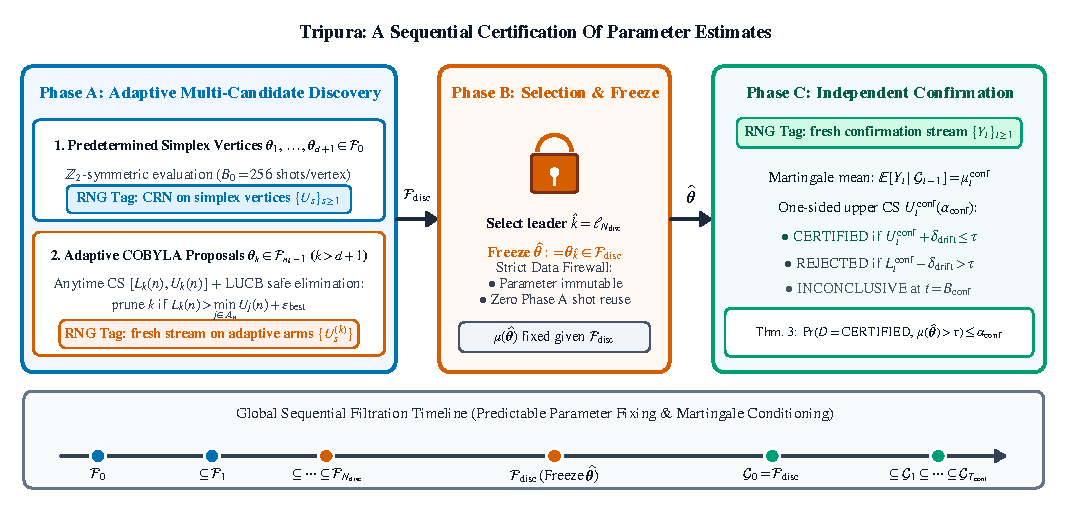
\includegraphics[width=\linewidth]{figures/fig1_architecture.pdf}
  \caption{The three phases of Tripura. Phase~A runs adaptive search within a budget $\Bdisc$. Phase~B freezes $\thhat$ at no shot cost and starts a new filtration $\G_0 = \Fdisc$. Phase~C tests $\thhat$ on a fresh stream up to a cap $\Bconf$ and stops early to certify or reject using anytime-valid confidence sequences at level $\aconf$.}
  \label{fig:architecture}
\end{figure}

\noindent\fbox{\parbox{0.97\linewidth}{\small
\textbf{Protocol: Tripura.} \emph{Inputs:} threshold $\tau$; budgets $\Bdisc, \Bconf$; pool cap $\Kmax$; error levels $\adisc$ and $\aup + \alow \le \aconf$; tolerance $\epsbest$; drift bound $\ddrift \ge 0$ (zero if stationary).
\begin{enumerate}
  \item[\textbf{A.}] Fix the initial simplex $\th_1, \dots, \th_{d+1}$ and give every candidate $k$ a pre-assigned error level $\alpha_k$ with $\textstyle\sum_{k\le \Kmax} \alpha_k \le \adisc$. Repeat until $\Bdisc$ is used up: let the optimizer propose new candidates (each starts with a small pilot batch); keep a confidence sequence $[L_k, U_k]$ for every active candidate; take the empirical leader $\ell$; eliminate any $k$ with $L_k > \min_j U_j + \epsbest$; stop if one candidate remains or $U_\ell \le \min_{j\neq\ell} L_j + \epsbest$; otherwise measure the leader and its strongest challenger (LUCB).
  \item[\textbf{B.}] Freeze $\thhat = \th_\ell$ and discard all Phase~A data for the purpose of certification. This uses no shots.
  \item[\textbf{C.}] Draw fresh shots at $\thhat$ from a seed independent of Phase~A, in batches of $b_{\mathrm{conf}}$. After each batch update $U_t^{\mathrm{conf}}$ (level $\aup$) and $L_t^{\mathrm{conf}}$ (level $\alow$). Output \textup{\textsc{Certified}} if $U_t^{\mathrm{conf}} + \ddrift \le \tau$, \textup{\textsc{Rejected}} if $L_t^{\mathrm{conf}} - \ddrift > \tau$, and \textup{\textsc{Inconclusive}} if $\Bconf$ is reached first.
\end{enumerate}
\emph{Output:} $\thhat$, the decision, the final interval, and the total shot count $\Ndisc + \Nconf$.
}}

\bigskip\noindent\textbf{What the guarantees need.} The Phase~C guarantee needs only the freeze, a fresh stream, and the stopping rule above. The Phase~A guarantee additionally needs fixed per-candidate error levels, fresh streams on adaptive candidates, and the elimination rule as stated. In the experiments, Phase~A also used two accelerations that the proof of Theorem~\ref{thm:elimination} does not cover: Holm-style recycling of error levels as candidates are eliminated, and pairwise-difference betting against the current leader. We report their effect separately in Section~\ref{sec:res_cost}. Phase~C validity does not depend on them.

\section{Theoretical guarantees}
\label{sec:theory}

Candidates $\th_1, \dots, \th_K$ ($K \ge 2$) have risks $\mu_k$, $\mu_\star = \min_k \mu_k$, and each is estimated by an unbiased $\widehat\mu_k \in [0, 1]$ from a deterministic number $B_k$ of shots. Let $\hat k$ be the smallest index minimizing $\widehat\mu_k$ and $k_\star$ a true minimizer.

\medskip\noindent\textbf{Theorem 1} (Selection optimism and in-sample certification).\label{thm:selection_bias}
\begin{enumerate}
  \item[\emph{(a)}] \emph{\textbf{Sign and strictness.} Without any independence across candidates,}
  \begin{equation}
    \E[\widehat\mu_{\hat k} - \mu_{\hat k}]
    = \bigl(\E[\min_k \widehat\mu_k] - \mu_\star\bigr) - \E[\mu_{\hat k} - \mu_\star]
    \le -\E\bigl[(\widehat\mu_{k_\star} - \min_{j\neq k_\star}\widehat\mu_j)_+\bigr] \le 0.
    \label{eq:selection_decomposition}
  \end{equation}
  \emph{The bias is strictly negative if and only if $\Prob(\min_{j\neq k_\star}\widehat\mu_j < \widehat\mu_{k_\star}) > 0$ or $\Prob(\mu_{\hat k} > \mu_\star) > 0$.}
  \item[\emph{(b)}] \emph{\textbf{Finite-sample bound.} If the errors $Z_k = \mu_k - \widehat\mu_k$ are sub-Gaussian with variance proxy $v_k / B_k$ (true with $v_k = 1/4$ for means of $B_k$ conditionally independent $[0, 1]$ shots \cite{hoeffding1963}), then under any coupling across candidates}
  \begin{equation}
    0 \le \E[\mu_{\hat k} - \widehat\mu_{\hat k}]
    \le \E\bigl[\max_k Z_k\bigr]
    \le \sqrt{2\ln K \max_k \frac{v_k}{B_k}}.
    \label{eq:selection_bound}
  \end{equation}
  \item[\emph{(c)}] \emph{\textbf{In-sample certification.} Let $U_k = \widehat\mu_k + r_k$ be upper bounds with $\Prob(U_k \le \tau) = p_k$ when $\mu_k > \tau$, and suppose all candidates are infeasible. Then}
  \begin{equation}
    \Prob(U_{\hat k} \le \tau) \le \Prob\bigl(\min_k U_k \le \tau\bigr).
    \label{eq:insample_partition}
  \end{equation}
  \emph{If all radii are equal, or the candidate with the smallest $U_k$ is selected, the two events coincide, and for independent $\widehat\mu_k$,}
  \begin{equation}
    \Prob\bigl(\min_k U_k \le \tau\bigr) = 1 - \prod_{k=1}^K (1 - p_k).
    \label{eq:insample_product}
  \end{equation}
\end{enumerate}

Part~(b) is the standard maximal inequality for sub-Gaussian variables \cite{massart2007}; the point is that it applies to the \emph{selected} candidate with arbitrary coupling. Equation~\eqref{eq:insample_product} says that testing $K$ infeasible candidates at level $\alpha$ each and keeping the best one certifies a false claim with probability close to $1 - (1 - \alpha)^K$.

\medskip\noindent\emph{Remark 3 (Boundary cases).}\label{rem:boundary_cases}
The inequality in~(a) is not always strict. For $K = 2$, $X_1 \sim \mathrm{Unif}(0, 0.1)$ and $X_2 \sim \mathrm{Unif}(0.2, 0.3)$ with one shot each, $\hat k = 1$ almost surely and the bias is exactly zero. When means are equal and errors Gaussian, the bias is $-c_K\sigma/\sqrt{B}$ with $c_K = \E[\max_k \xi_k] \le \sqrt{2\ln K}$ for standard normal $\xi_k$, so the $\sqrt{\ln K}$ growth in~\eqref{eq:selection_bound} is the right order. For~(c), with unequal radii the winner by empirical mean need not minimize $U_k$: with $\tau = 0.20$, $(\widehat\mu_1, r_1) = (0.10, 0.15)$ and $(\widehat\mu_2, r_2) = (0.12, 0.05)$, candidate~1 wins but $U_1 = 0.25 > \tau \ge U_2 = 0.17$. Finally, (b) assumes fixed $B_k$; if $B_k$ is itself a data-dependent stopping time, optional-stopping effects add to the bias, which is why Phase~A uses time-uniform confidence sequences.

\subsection{Confidence sequences and Phase A}
\label{subsec:cs_phaseA}

For each candidate we use time-uniform confidence sequences that are imported from the literature: a stitched empirical-Bernstein construction \cite{howard2021} and a hedged-betting construction \cite{waudby2024} (Appendix~\ref{app:cs_used}).

\medskip\noindent\textbf{Proposition 1} (Imported \cite{howard2021,waudby2024}).\label{prop:cs_validity}
\emph{Let $X_1, X_2, \dots \in [0, 1]$ satisfy $\E[X_s \mid \Hfil_{s-1}] = \mu$ for a filtration $(\Hfil_s)$. For levels $\alpha_{\mathrm{low}}, \alpha_{\mathrm{high}} > 0$ the empirical-Bernstein and betting constructions each give $[L_t, U_t]$ with $\Prob(\exists t : \mu < L_t) \le \alpha_{\mathrm{low}}$ and $\Prob(\exists t : \mu > U_t) \le \alpha_{\mathrm{high}}$.}

\medskip
The proof is that, at the true mean, the relevant processes are nonnegative supermartingales started at one, and Ville's inequality \cite{ville1939} bounds their supremum. Evaluating betting sets on a finite grid of means is made conservative by widening the interval by one grid cell on each side.

\medskip\noindent\textbf{Theorem 2} (Simultaneous coverage and safe elimination).\label{thm:elimination}
\emph{Assume~\eqref{eq:validity_condition} holds for each candidate stream (Mode~U, or Mode~H using Remark~2). At most $\Kmax$ candidates are created, candidate $k$ gets level $\alpha_k$ with $\textstyle\sum_k \alpha_k \le \adisc$, and the elimination and stopping rules of the protocol are used with $\ell_n$ the empirical leader. Let $\mu_\star$ be the best risk among candidates created by the stopping time $\Ndisc$. Then with probability at least $1 - \adisc$:}
\begin{enumerate}
  \item[\emph{(a)}] \emph{$\mu_k \in [L_k(n), U_k(n)]$ for every candidate $k$ and every $n \le \Ndisc$;}
  \item[\emph{(b)}] \emph{every candidate with $\mu_k \le \mu_\star + \epsbest$ stays active throughout, in particular no true minimizer is eliminated;}
  \item[\emph{(c)}] \emph{if discovery stops before $\Bdisc$ through the rules above, the selected candidate satisfies $\mu_{\hat k} \le \mu_\star + \epsbest$.}
\end{enumerate}

\medskip\noindent\emph{Remark 4 (Scope of Theorem~2).}\label{rem:scope_thm2}
The guarantee is relative to the finite pool the optimizer actually generated. Whether COBYLA proposes a parameter near the global optimum of a non-convex objective is an empirical question. The leader is never eliminated. The theorem does not cover Mode~C, nor the Holm-recycling and pairwise-betting accelerations mentioned in Section~\ref{sec:model}; we test those empirically.

\subsection{Freezing and certification}
\label{subsec:freezing_certification}

After Phase~B the frozen $\thhat$ is $\Fdisc$-measurable. Phase~C draws fresh shots $\widetilde X_1, \widetilde X_2, \dots \in [0, 1]$, generating $\G_t = \sigma(\Fdisc, \widetilde X_1, \dots, \widetilde X_t)$, with $\E[\widetilde X_t \mid \G_{t-1}] = \mu(\thhat)$. Let $U_t^{\mathrm{conf}}$ and $L_t^{\mathrm{conf}}$ be one-sided sequences from Proposition~1 at levels $\aup$ and $\alow$ with $\aup + \alow \le \aconf$. The decision is \textup{\textsc{Certified}} at the first $t \le \Bconf$ with $U_t^{\mathrm{conf}} \le \tau$, \textup{\textsc{Rejected}} at the first $t$ with $L_t^{\mathrm{conf}} > \tau$ (whichever comes first), and \textup{\textsc{Inconclusive}} otherwise.

\medskip\noindent\textbf{Theorem 3} (End-to-end certification).\label{thm:conf}
\emph{Let $\thhat \in \Fdisc$ be produced by any Phase~A procedure (Mode~U, H or C).}
\begin{enumerate}
  \item[\emph{(a)}] \emph{\textbf{Type-I error.} Almost surely,}
  \begin{equation}
    \Prob(D = \textup{\textsc{Certified}} \mid \Fdisc)\,\ind[\mu(\thhat) > \tau]
    \le \aup\,\ind[\mu(\thhat) > \tau],
    \label{eq:cond_typeI}
  \end{equation}
  \emph{and therefore $\Prob(D = \textup{\textsc{Certified}},\; \mu(\thhat) > \tau) \le \aup \le \aconf$. This holds regardless of selection bias and of how CRN was used in Phase~A.}
  \item[\emph{(b)}] \emph{\textbf{Joint guarantee.} If Phase~A satisfies Theorem~2, then with probability at least $1 - \adisc - \aconf$ no $\epsbest$-optimal candidate is eliminated and no infeasible parameter is certified.}
\end{enumerate}

\medskip\noindent\emph{Remark 5 (Scope and drift).}\label{rem:scope_thm3}
Part~(a) is a statement about error probability, not power: a feasible candidate can still end \textup{\textsc{Inconclusive}}. Conditional independence of shots is not needed, only the conditional-mean condition. If several frozen candidates are tested in turn with levels summing to at most $\aconf$, the familywise false-certification probability is at most $\aconf$. For the betting construction, a bounded readout drift $|\E[\widetilde X_t \mid \G_{t-1}] - \mu(\thhat)| \le \ddrift$, with $\ddrift$ known, is handled by certifying only when $U_t^{\mathrm{conf}} + \ddrift \le \tau$ (and rejecting only when $L_t^{\mathrm{conf}} - \ddrift > \tau$): the betting process evaluated at $\mu(\thhat) - \ddrift$ is still a nonnegative supermartingale (Appendix~\ref{app:proofs}). The drift bound must be known; we do not claim anything for unknown or unbounded drift.

\section{Experimental design}
\label{sec:exp_design}

All experiments use exact statevector simulation of QAOA MaxCut with genuine multinomial shot sampling. No quantum hardware was used.

\paragraph*{Instances.}
Every instance is a connected, non-isomorphic, unweighted 3-regular graph evaluated with depth $p = 2$ QAOA ($d = 4$ parameters, $5$ initial simplex vertices), warm-started from the Wurtz--Love 3-regular angles with random jitter. The thresholds $\tau_{12} = 0.261891$ and $\tau_{14} = 0.268661$ were fixed on a separate calibration ensemble before either study and never changed. The two studies below use disjoint sets of graphs.

\paragraph*{Selection-bias study (100 graphs, 300 trajectories per cell).}
$50$ graphs at $n = 12$ and $50$ at $n = 14$, three optimizer repetitions each. We run COBYLA and, for prefix lengths $K \in \{1, 25, 50, 100\}$ and per-candidate budgets $B \in \{256, 512, 1024, 2048\}$, select $\hat k = \arg\min_{k\le K} \widehat\mu_k$. We then re-evaluate the selected candidate on an independent stream of $4096$ shots.

\paragraph*{End-to-end study (500 graphs: 80 at $n = 12$, 420 at $n = 14$).}
One trajectory per graph. Discovery cap $\Bdisc = 2560$, confirmation cap $\Bconf = 4096$, $\epsbest = 0.008$, $\adisc = \aconf = 0.05$; $10$ further graphs were used only to freeze hyperparameters. The confirmation sampler uses a seed disjoint from all Phase~A seeds in every mode. The Phase~A and Phase~C procedures use the betting confidence sequence. $\Kmax = 10$ in Modes~U, H and~C.

\paragraph*{Modes and baselines at matched discovery budget (Table~\ref{tab:modes_setup}).}
Table~\ref{tab:modes_setup} summarizes the experimental modes and matched-budget baselines evaluated on the 500-graph benchmark ($\Bdisc = 2560$, $\Bconf = 4096$, $\adisc = \aconf = 0.05$).
\begin{enumerate}
  \item \emph{Uniform + fixed-4096:} COBYLA with uniform shot allocation over $16$ candidates ($2560$ shots), then one fixed-horizon 4096-shot confirmation at $\aconf = 0.05$ ($6656$ shots in total).
  \item \emph{Uniform + sequential (EB and betting):} the same discovery, followed by sequential confirmation (batch $256$, cap $4096$) evaluated both with the Howard Gamma-Exponential empirical-Bernstein sequence and with the same hedged-betting sequence used by Modes~U, H and~C (Section~\ref{sec:res_cost}).
\end{enumerate}

\begin{table}[!htbp]
  \caption{Experimental modes and matched-budget baselines in the 500-graph end-to-end study ($80$ graphs at $n=12$, $420$ at $n=14$; QAOA depth $p=2$, $\Bdisc = 2560$, $\Bconf = 4096$, $\adisc = \aconf = 0.05$). In Modes~U, H and~C, Phase~A initializes $d+1=5$ simplex vertices ($256$ shots each), allocates $128$ pilot shots to new COBYLA proposals ($\Kmax = 10$), and races active candidates in batches of $32$ shots.}
  \label{tab:modes_setup}
  \centering
  \resizebox{\linewidth}{!}{%
  \begin{tabular}{llllll}
    \toprule
    Method / Mode & Phase~A RNG regime & Phase~A allocation \& CS & Phase~C confirmation ($b_{\mathrm{conf}}=256$) & Phase~A guarantee & Phase~C guarantee \\
    \midrule
    Uniform + fixed-4096           & Independent streams           & Uniform ($16 \times 160$ shots) & Fixed $4096$ shots (EB)          & n/a (no elimination)           & Guaranteed ($\le \aconf$) \\
    Uniform + sequential (EB)      & Independent streams           & Uniform ($16 \times 160$ shots) & Sequential Gamma-Exp.\ EB        & n/a (no elimination)           & Guaranteed ($\le \aconf$) \\
    Uniform + sequential (betting) & Independent streams           & Uniform ($16 \times 160$ shots) & Sequential hedged betting        & n/a (no elimination)           & Guaranteed ($\le \aconf$) \\
    Mode~U (deployable)            & Independent streams (all $k$) & LUCB racing + hedged betting    & Sequential hedged betting        & Guaranteed (Thm.~\ref{thm:elimination})\textsuperscript{a} & Guaranteed ($\le \aconf$) \\
    Mode~H (simulation)            & CRN on $5$ simplex vertices   & LUCB racing + hedged betting    & Sequential hedged betting        & Guaranteed (Rem.~2)\textsuperscript{a} & Guaranteed ($\le \aconf$) \\
    Mode~C (ablation)              & Full CRN reuse across all $k$ & LUCB racing + hedged betting    & Sequential hedged betting        & Not guaranteed (Rem.~2)        & Guaranteed ($\le \aconf$) \\
    \bottomrule
  \end{tabular}}
  \vspace{0.2em}
  \par\noindent\scriptsize\textsuperscript{a}Theorem~\ref{thm:elimination} covers the pre-allocated schedule $\alpha_k = \adisc/\Kmax$ (audited in \texttt{C1}/\texttt{C2}); the 500-graph runs also enable Holm recycling and pairwise-betting racing accelerations (Section~\ref{sec:res_cost}).
\end{table}

\paragraph*{Statistics.}
Proportions carry Clopper--Pearson intervals \cite{clopper1934} (one-sided $95\%$ upper bounds when no events occur). Continuous quantities are mean $\pm$ standard error over graphs. Paired tests use Holm adjustment \cite{holm1979}.

\section{Results}
\label{sec:results}

\subsection{Selection bias is real and matches the bound}
\label{sec:res_bias}

Table~\ref{tab:selection_bias} and Fig.~\ref{fig:selection_bias} show the in-sample bias $\widehat\mu_{\hat k} - \mu(\thhat)$. At $K = 1$ there is no selection and the bias is zero within error. For $K > 1$ it is negative, grows with $\ln K$, and shrinks roughly as $B^{-1/2}$: at $B = 256$ it reaches $-0.0124 \pm 0.0003$ for $K = 100$, and at $B = 2048$ it is smaller by a factor of $2.88 \approx \sqrt{8}$. In all $12$ multi-candidate cells the observed bias lies below the bound~\eqref{eq:selection_bound} with $v_k = 1/4$, by a factor between $7.5$ and $8.5$. This bound is conservative because the real per-shot variance of the QAOA loss is much smaller than $1/4$. Re-evaluating the frozen winner on a fresh 4096-shot stream removes the bias in every cell ($|\text{bias}| \le 0.0002$).

\begin{table}[!htbp]
  \caption{Selection bias versus fresh-confirmation bias (100 graphs, 300 trajectories per cell; mean $\pm$ SE). The bound is $\sqrt{2\ln K / (4B)}$ from Eq.~\eqref{eq:selection_bound} with $v_k = 1/4$. Results for $B \in \{512, 1024\}$ lie between these two rows and show the same pattern.}
  \label{tab:selection_bias}
  \centering
  \small
  \begin{tabular}{rrccc}
    \toprule
    $B$ & $K$ & In-sample bias $\widehat\mu_{\hat k} - \mu(\thhat)$ & Fresh-stream bias ($\Bconf = 4096$) & Bound ($v = 1/4$) \\
    \midrule
    256 & 1   & $+0.0001 \pm 0.0003$ & $-0.0001 \pm 0.0001$ & $0.0000$ \\
    256 & 25  & $-0.0099 \pm 0.0003$ & $+0.0000 \pm 0.0001$ & $0.0793$ \\
    256 & 50  & $-0.0117 \pm 0.0003$ & $-0.0000 \pm 0.0001$ & $0.0874$ \\
    256 & 100 & $-0.0124 \pm 0.0003$ & $+0.0001 \pm 0.0001$ & $0.0948$ \\
    \midrule
    2048 & 1   & $+0.0001 \pm 0.0001$ & $-0.0000 \pm 0.0001$ & $0.0000$ \\
    2048 & 25  & $-0.0033 \pm 0.0001$ & $-0.0000 \pm 0.0001$ & $0.0280$ \\
    2048 & 50  & $-0.0040 \pm 0.0001$ & $-0.0001 \pm 0.0001$ & $0.0309$ \\
    2048 & 100 & $-0.0043 \pm 0.0001$ & $+0.0002 \pm 0.0001$ & $0.0335$ \\
    \bottomrule
  \end{tabular}
\end{table}

\begin{figure}[!htbp]
  \centering
  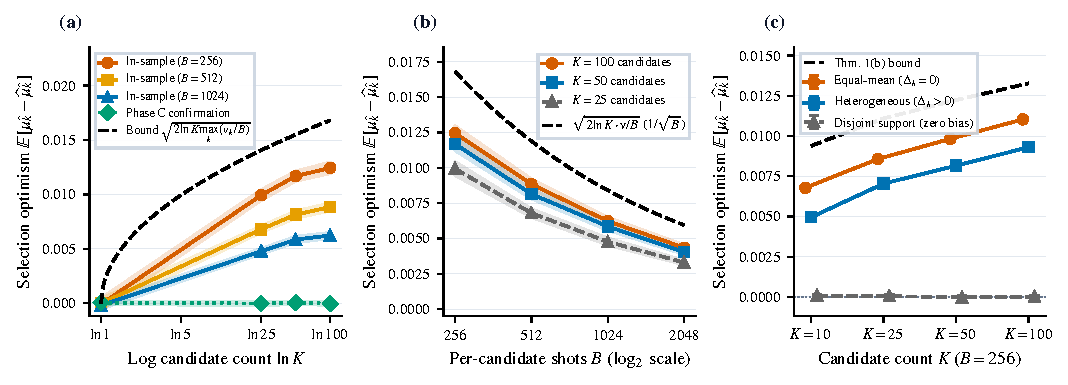
\includegraphics[width=\linewidth]{figures/fig2_selection_bias.pdf}
  \caption{Post-selection optimism (Theorem~1(a,b)). (a)~Bias magnitude versus pool size $K$ for several per-candidate budgets $B$, with the sub-Gaussian envelope (dashed). (b)~Decay with $B$ on log--log axes, consistent with $B^{-1/2}$. (c)~Synthetic check of Remark~3: equal-mean candidates follow the order-statistic scale, while candidates with disjoint noise supports show zero bias.}
  \label{fig:selection_bias}
\end{figure}

\subsection{Why the candidate must be frozen}
\label{sec:res_freeze}

Table~\ref{tab:insample_vs_frozen} and Fig.~\ref{fig:insample_vs_frozen} compare certification on the discovery data with certification on a frozen candidate (budget $B = 256$, nominal level $0.05$). A standard Student-$t$ upper bound computed on the discovery data covers the true risk $\mu(\thhat)$ in $94.7\%$ of cases at $K = 1$, but only $34.3\%$, $9.3\%$ and $6.0\%$ at $K = 25, 50$ and $100$. In other words, the stated confidence level stops meaning anything once a winner has been selected. On this benchmark the false-certification rate rises to $0.050$ at $K = 100$, from $0.003$ at $K = 1$; it reaches the nominal level rather than clearly exceeding it, because only a minority of selected winners are infeasible and close to the threshold. The collapse in coverage is the more informative sign. An in-sample Bonferroni correction with empirical-Bernstein radii avoids false certifications but almost never certifies anything ($0.000$ at $K = 100$), because the radii are very wide at $B = 256$. The frozen Phase~C confirmation certifies $58.3\%$ of trajectories at $K = 100$ with no false certifications and full coverage.

\begin{table}[!htbp]
  \caption{In-sample certification versus frozen independent confirmation ($B = 256$, nominal level $0.05$, 300 trajectories per row). False-cert.\ rate with exact $95\%$ Clopper--Pearson intervals; ``coverage'' is the fraction of trajectories with $\mu(\thhat) \le$ the upper bound. Frozen confirmation uses 4096 fresh shots and an empirical-Bernstein bound.}
  \label{tab:insample_vs_frozen}
  \centering
  \small
  \begin{tabular}{rlccc}
    \toprule
    $K$ & Method & Cert.\ rate & False-cert.\ rate [$95\%$ CP] & Coverage \\
    \midrule
    1   & In-sample Student-$t$       & 0.497 & 0.003 [0.000, 0.018] & 0.947 \\
    1   & In-sample Bonferroni EB     & 0.007 & 0.000 [0.000, 0.012] & 1.000 \\
    1   & Frozen Phase~C (EB)         & 0.567 & 0.000 [0.000, 0.012] & 1.000 \\
    \midrule
    25  & In-sample Student-$t$       & 0.700 & 0.023 [0.009, 0.047] & 0.343 \\
    25  & In-sample Bonferroni EB     & 0.003 & 0.000 [0.000, 0.012] & 1.000 \\
    25  & Frozen Phase~C (EB)         & 0.567 & 0.000 [0.000, 0.012] & 1.000 \\
    \midrule
    50  & In-sample Student-$t$       & 0.723 & 0.040 [0.021, 0.069] & 0.093 \\
    50  & In-sample Bonferroni EB     & 0.000 & 0.000 [0.000, 0.012] & 1.000 \\
    50  & Frozen Phase~C (EB)         & 0.577 & 0.000 [0.000, 0.012] & 1.000 \\
    \midrule
    100 & In-sample Student-$t$       & 0.753 & 0.050 [0.028, 0.081] & 0.060 \\
    100 & In-sample Bonferroni EB     & 0.000 & 0.000 [0.000, 0.012] & 1.000 \\
    100 & Frozen Phase~C (EB)         & 0.583 & 0.000 [0.000, 0.012] & 1.000 \\
    \bottomrule
  \end{tabular}
\end{table}

\begin{figure}[!htbp]
  \centering
  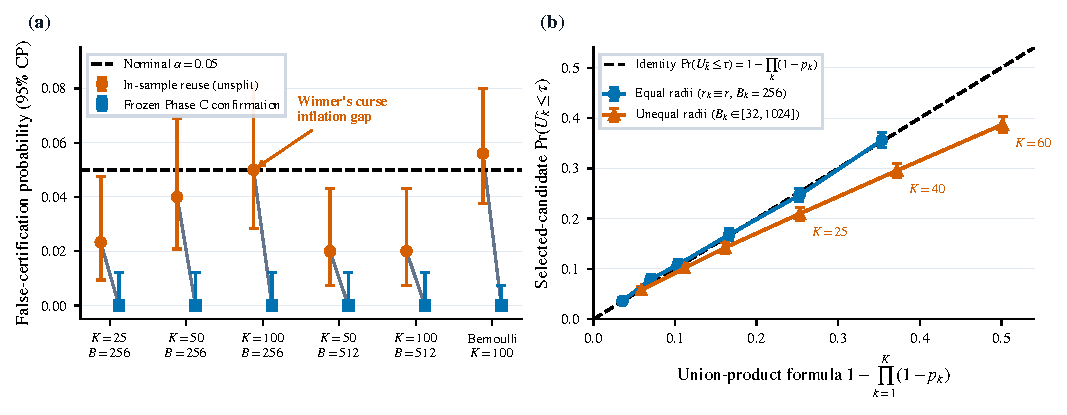
\includegraphics[width=\linewidth]{figures/fig3_insample_vs_independent.pdf}
  \caption{Failure of in-sample certification (Theorem~1(c)). (a)~False-certification rates with $95\%$ Clopper--Pearson bars for in-sample reuse versus frozen Phase~C confirmation; the dashed line is $0.05$. (b)~Synthetic check of Eqs.~\eqref{eq:insample_partition}--\eqref{eq:insample_product}: the false-certification probability falls on the diagonal $1 - \prod_k (1 - p_k)$ for equal radii and below it when radii differ.}
  \label{fig:insample_vs_frozen}
\end{figure}

\subsection{Phase C error control}
\label{sec:res_error_control}

In the 500-graph study at $\aconf = 0.05$, the frozen candidate was infeasible ($\mu(\thhat) > \tau_n$, so a false certification was possible) on $157$ graphs for Mode~U, $150$ for Mode~H, $128$ for Mode~C and $174$ for the uniform baselines. Phase~C certified none of them: $0/500$ false certifications in every method (one-sided $95\%$ Clopper--Pearson upper bound $0.0060$ over all graphs, and $0.0189$ and $0.0198$ over the at-risk graphs of Modes~U and~H). We repeated the evaluation at $\aconf \in \{0.01, 0.02, 0.03, 0.04, 0.05\}$ with both sequential and fixed confirmation and again found no false certification.

This benchmark is a weak test of the boundary: because the gap $|\mu(\thhat) - \tau_n|$ is rarely below about $10^{-3}$, few frozen candidates sit very close to the threshold. For this reason we added three stress tests, all run on synthetic confirmation streams or modified settings, not on the main benchmark.
\begin{enumerate}
  \item \emph{Boundary.} On $1000$ synthetic streams with $\mu(\thhat) = \tau + 10^{-4}$, sequential confirmation falsely certified between $0.0\%$ and $0.2\%$ of runs for $\aconf \in [0.01, 0.05]$, below the nominal level.
  \item \emph{Drift.} With a downward drift of $\ddrift = 0.005$ (stream mean below $\tau$ while $\mu(\thhat)$ is just above it), the unshifted rule falsely certified $58.0\%$ of $1000$ runs (betting) and $83.5\%$ (Gamma-Exponential EB). The shifted rule $U_t^{\mathrm{conf}} + \ddrift \le \tau$ gave $0/1000$ for both. The EB result is empirical only; the proof in Appendix~\ref{app:proofs} covers the betting construction.
  \item \emph{Readout noise.} On $60$ graphs with bit-flip readout noise $p_{\mathrm{err}} = 0.02$ and $0.05$, the effective risk of the selected circuit rose from $0.2612$ to $0.2667$ and $0.2744$. The certification rate fell from $0.450$ to $0.317$ and $0.183$ while rejections rose from $0.250$ to $0.433$ and $0.600$, with $0/60$ false certifications in each case.
\end{enumerate}

\subsection{Measurement cost and the effect of each component}
\label{sec:res_cost}

Table~\ref{tab:e2e} and Fig.~\ref{fig:cost_quality} give the end-to-end results at matched discovery budget. We separate three effects.

\begin{table}[!htbp]
  \caption{End-to-end comparison at matched discovery budget $\Bdisc = 2560$ ($G = 500$ graphs, mean $\pm$ SE). ``Best-ID'' is the fraction of graphs where the selected candidate is the best of the pool, ``$\epsbest$-ID'' where it is within $\epsbest$ of the best. ``Cert.'' is the fraction of graphs certified; ``false certs'' counts certifications of infeasible candidates. Approximation ratio is $\langle C\rangle_{\thhat} / C_{\max}$. Mode~H and~C are simulation-only.}
  \label{tab:e2e}
  \centering
  \resizebox{\linewidth}{!}{%
  \begin{tabular}{lcccccccccc}
    \toprule
    Method & Disc.\ shots & Conf.\ shots & Total shots & Saved & Best-ID & $\epsbest$-ID & Cert. & False certs & Approx.\ ratio \\
    \midrule
    Uniform + fixed-4096          & $2560$          & $4096$            & $6656$            & $0.0\%$  & $0.008$ & $0.738$ & $0.532$ & $0/500$ & $0.8464$ \\
    Uniform + sequential (EB)     & $2560$          & $1733.6 \pm 65.2$ & $4293.6 \pm 65.2$ & $35.5\%$ & $0.008$ & $0.738$ & $0.536$ & $0/500$ & $0.8464$ \\
    Uniform + sequential (betting)& $2560$          & $1457.2 \pm 67.5$ & $4017.2 \pm 67.5$ & $39.6\%$ & $0.008$ & $0.738$ & $0.544$ & $0/500$ & $0.8464$ \\
    Mode~U (deployable)           & $1979.8 \pm 36.3$ & $1351.7 \pm 66.2$ & $3331.5 \pm 89.2$ & $49.9\%$ & $0.398$ & $0.878$ & $0.580$ & $0/500$ & $0.8466$ \\
    Mode~H (simulation)           & $1955.9 \pm 36.9$ & $1242.6 \pm 64.7$ & $3198.5 \pm 86.8$ & $51.9\%$ & $0.486$ & $0.946$ & $0.610$ & $0/500$ & $0.8481$ \\
    Mode~C (ablation)             & $1982.8 \pm 37.6$ & $1081.9 \pm 57.5$ & $3064.6 \pm 79.3$ & $54.0\%$ & $0.718$ & $0.992$ & $0.664$ & $0/500$ & $0.8493$ \\
    \bottomrule
  \end{tabular}}
\end{table}

\paragraph*{Sequential confirmation alone.}
Replacing the fixed 4096-shot confirmation by sequential confirmation after the same uniform discovery reduces total shots from $6656$ to $4293.6 \pm 65.2$ ($35.5\%$ saved) with the empirical-Bernstein sequence and to $4017.2 \pm 67.5$ ($39.6\%$ saved) with the betting sequence, with an unchanged candidate and no loss in certification rate ($0.536$ and $0.544$ versus $0.532$).

\paragraph*{Phase A racing.}
Racing with confidence-sequence elimination used $1979.8 \pm 36.3$ discovery shots in Mode~U instead of $2560$, about $23\%$ fewer, and picked a better candidate: best-candidate identification rose from $0.008$ to $0.398$ and $\epsbest$-identification from $0.738$ to $0.878$. The mean true risk of the chosen candidate was not significantly different from that of uniform discovery in Mode~U ($-0.00029 \pm 0.00028$, $p_{\mathrm{Holm}} = 0.301$), so the approximation ratio is essentially unchanged ($0.8466$ versus $0.8464$). The honest summary for the deployable protocol is therefore that it reaches the same solution quality with fewer shots, not a better one. Mode~U uses $962.1 \pm 66.0$ fewer total shots than \emph{Uniform + sequential (EB)} (paired $p_{\mathrm{Holm}} = 6.95 \times 10^{-40}$) and $685.6 \pm 67.7$ fewer total shots than \emph{Uniform + sequential (betting)} using the identical confirmation engine (paired $t$-test $p = 4.75 \times 10^{-22}$, Wilcoxon $p = 4.61 \times 10^{-25}$). The certification rate rose from $0.536$ ($0.544$ under betting) to $0.580$.

\begin{figure}[!htbp]
  \centering
  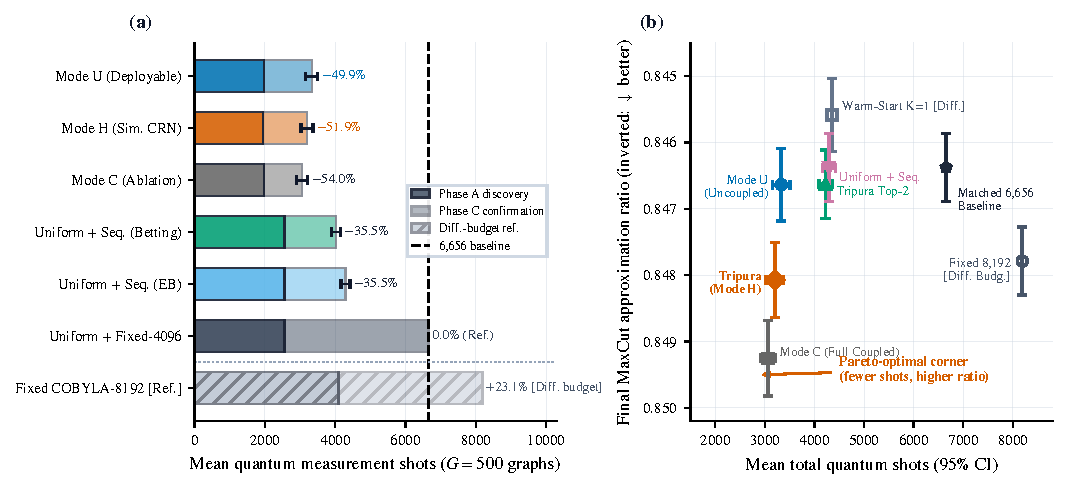
\includegraphics[width=\linewidth]{figures/fig6_cost_and_quality.pdf}
  \caption{End-to-end cost and quality over 500 graphs. (a)~Mean discovery and confirmation shots relative to the 6,656-shot fixed-confirmation baseline (dashed line). (b)~Total shots versus final approximation ratio $\langle C\rangle_{\thhat} / C_{\max}$ ($\pm 1\;\mathrm{SE}$).}
  \label{fig:cost_quality}
\end{figure}

\paragraph*{Isolating the confirmation engine from Phase A racing.}
Comparing \emph{Uniform + sequential (EB)} ($4293.6 \pm 65.2$ total shots) against \emph{Uniform + sequential (betting)} ($4017.2 \pm 67.5$ total shots) on the exact same Phase~A discovery trajectories shows that switching the Phase~C engine from empirical-Bernstein to betting accounts for $276.5$ confirmation shots. Holding the betting confirmation engine fixed across both pipelines, Phase~A racing in Mode~U saves $685.6 \pm 67.7$ total shots ($580.2 \pm 36.3$ in discovery and $105.5 \pm 54.5$ in confirmation) while substantially improving within-pool candidate identification.

\paragraph*{Simplex CRN (simulation only).}
Using CRN on the $5$ initial vertices (Mode~H) gave a lower true risk than Mode~U ($-0.00129 \pm 0.00021$, $p_{\mathrm{Holm}} = 4.8 \times 10^{-9}$), higher identification ($0.486$ versus $0.398$) and a higher approximation ratio ($0.8481$). The saving of $133.0 \pm 65.4$ shots over Mode~U is small and not robust ($p = 0.043$ for the paired $t$-test, $0.085$ for the Wilcoxon test), so we do not claim a shot saving from CRN. Phase~A empirical coverage in Mode~H was $0.998$.

\paragraph*{Full CRN (Mode C).}
Mode~C had the highest identification accuracy and the fewest shots, but its Phase~A guarantee is void by Remark~2: reusing the draws that steered the search makes the conditional mean of later shots differ from $\mu(\th_k)$. We include Mode~C only as an ablation; its good performance must not be read as validity. Phase~C error control is unaffected: $0/500$ false certifications.

\paragraph*{Phase A safety audit.}
The proof of Theorem~2 covers the pre-allocated schedule $\alpha_k = \adisc / \Kmax$ without Holm recycling or pairwise betting. On a 50-graph validation suite this schedule had $1.000$ coverage and no wrongful elimination with simplex CRN ($2194.6$ discovery shots) and with uncoupled streams ($2175.4$). With Holm recycling and pairwise betting, Mode~H used $2058.9$ discovery shots, again with $1.000$ coverage and $0/50$ wrongful eliminations. The accelerations therefore saved about $136$ shots without any observed loss of safety, but only the pre-allocated schedule is covered by the theorem.

\section{Limitations and next steps}
\label{sec:limitations}

\paragraph*{Simulation only.}
All numbers come from exact statevector simulation of 12- and 14-qubit, depth-2 QAOA on unweighted 3-regular MaxCut. We had no access to quantum hardware, and the available classical compute did not allow larger instances, deeper circuits, or many trajectories per graph (each graph has one trajectory in the end-to-end study). Real devices add drifting calibration, correlated readout errors and gate noise; our noise test models only independent bit-flips on readout. Running Tripura on hardware is the natural next step, and Mode~U is the version designed for it. CRN-based modes cannot be run on hardware at all.

\paragraph*{Scope of the guarantees.}
Theorem~2 holds relative to the candidates the optimizer actually proposes, not the global optimum. Theorem~3 controls the false-certification probability, not the power, and the drift extension requires a known bound $\ddrift$ obtained, for example, from device calibration. The thresholds $\tau_n$ were fixed on a calibration ensemble of the same graph family, so the certification rates (as opposed to the error rates) should not be assumed to transfer to other families. The Phase~A accelerations (Holm recycling, pairwise betting) are supported only by experiments.

\paragraph*{Baselines.}
We compared against fixed-horizon and uniform-allocation baselines at matched budget and against the adaptive-shot literature only qualitatively. Methods such as iCANS and Rosalin tackle a different problem (shot allocation along an optimization trajectory) and could be combined with Tripura as the proposer. A like-for-like comparison with other certification procedures was not run.

\paragraph*{Other estimators.}
The framework applies to any $[0, 1]$-bounded single-shot estimator, including Pauli-sampled VQE energies and holdout losses in quantum machine learning, but only the QAOA estimator was tested.

\section{Conclusion}
\label{sec:conclusion}

Selecting the best-looking parameters from a noisy search and then certifying them on the same data produces estimates that are biased downward and confidence statements that stop being valid. Tripura avoids this by separating discovery, a zero-shot freeze, and sequential confirmation on fresh data. The confirmation step controls the false-certification probability at the chosen level whatever Phase~A did. In simulation on 500 QAOA MaxCut instances the deployable version made no false certifications and used about half the shots of a fixed-confirmation baseline; roughly $35$--$40$ percentage points of that saving come from sequential stopping alone, and the remaining $\approx 10$ percentage points ($685.6 \pm 67.7$ shots under the matched betting engine) come from racing in discovery. Hardware experiments and larger-scale tests are the next step.

\section*{Acknowledgements}
The author thanks colleagues for helpful discussions on sequential inference and variational quantum optimization.

\section*{Data and code availability}
Simulation code, configuration files, raw trajectory logs and processed summary tables are available in the accompanying repository archive. All numerical results come from exact statevector simulations with simulated finite-shot multinomial sampling.

\appendix

\section{Proofs}
\label{app:proofs}

\subsection{Theorem 1}
\label{app:proof_thm1}

\noindent\textbf{(a)} Adding and subtracting $\mu_\star$ gives the pointwise identity $\widehat\mu_{\hat k} - \mu_{\hat k} = (\min_k \widehat\mu_k - \mu_\star) - (\mu_{\hat k} - \mu_\star)$, which gives the first equality in~\eqref{eq:selection_decomposition}. Since $\mu_{\hat k} \ge \mu_\star$, the second term is nonpositive in expectation. Next, $\min_k \widehat\mu_k = \widehat\mu_{k_\star} - (\widehat\mu_{k_\star} - \min_{j\neq k_\star}\widehat\mu_j)_+$, and unbiasedness $\E[\widehat\mu_{k_\star}] = \mu_\star$ gives $\E[\min_k \widehat\mu_k] - \mu_\star = -\E[(\widehat\mu_{k_\star} - \min_{j\neq k_\star}\widehat\mu_j)_+]$. Both terms of the bias are then expectations of nonnegative variables (with a minus sign), and such an expectation is positive exactly when the variable is positive with positive probability. This gives the strictness condition.

\noindent\textbf{(b)} Pointwise, $\mu_{\hat k} - \widehat\mu_{\hat k} = Z_{\hat k} \le \max_k Z_k$. Let $v_\star = \max_k v_k / B_k$. For $\lambda > 0$, by Jensen's inequality, $\exp(\lambda \E \max_k Z_k) \le \E \max_k e^{\lambda Z_k} \le \sum_k \E e^{\lambda Z_k} \le K e^{\lambda^2 v_\star / 2}$. Hence $\E \max_k Z_k \le \ln K / \lambda + \lambda v_\star / 2$, minimized at $\lambda = \sqrt{2\ln K / v_\star}$, which gives~\eqref{eq:selection_bound}. The lower bound $0 \le$ is part~(a).

\noindent\textbf{(c)} The events $\{\hat k = k\}$ partition the sample space, so $\Prob(U_{\hat k} \le \tau) = \sum_k \Prob(\hat k = k,\; \widehat\mu_k \le \tau - r_k)$. Since $U_{\hat k} \ge \min_k U_k$ pointwise, $\{U_{\hat k} \le \tau\} \subseteq \{\min_k U_k \le \tau\}$. With equal radii, $\hat k$ also minimizes $U_k$, so the events coincide; if $\tilde k$ minimizes $U_k$ they coincide by definition. For independent $\widehat\mu_k$, $\Prob(\min_k U_k \le \tau) = 1 - \prod_k \Prob(U_k > \tau) = 1 - \prod_k (1 - p_k)$.

\subsection{Proposition 1 and Theorem 2}
\label{app:proof_thm2}

\noindent\textbf{Proposition 1.} For the betting construction, the capital $K_t^\pm(\mu)$ is a product of factors with conditional mean one, bounded below by $1 - c > 0$, started at one, hence a nonnegative martingale. Ville's inequality bounds $\Prob(\exists t : K_t^+(\mu) \ge 1/\alpha_{\mathrm{low}}) \le \alpha_{\mathrm{low}}$, and likewise for $K_t^-$. For the empirical-Bernstein construction, Howard et al.\ \cite{howard2021} show that $\exp\{\lambda S_t - \psi_E(\lambda)\widehat V_t\}$ is a nonnegative supermartingale for $[0, 1]$-bounded increments with $\psi_E(\lambda) = -\ln(1 - \lambda) - \lambda$; stitching or mixing over $\lambda$ and applying Ville's inequality gives the claim.

\noindent\textbf{Theorem 2.} (a) Conditional on the history at which $\th_k$ is created, candidate $k$'s stream satisfies the hypothesis of Proposition~1 (by optional skipping in Mode~U and for adaptive candidates in Mode~H, and by Remark~2(i) for CRN-coupled vertices), so its miscoverage probability is at most $\alpha_k$; Boole's inequality over at most $\Kmax$ candidates gives total probability at most $\sum_k \alpha_k \le \adisc$. Work on the coverage event. (b) If $\mu_k \le \mu_\star + \epsbest$, then for every active $j$, $L_k(n) \le \mu_k \le \mu_\star + \epsbest \le \mu_j + \epsbest \le U_j(n) + \epsbest$, so $L_k(n) \le \min_j U_j(n) + \epsbest$ and $k$ is never eliminated. (c) A true minimizer $k_\star$ is active by~(b). If $|\mathcal{A}| = 1$ the leader is $k_\star$. Otherwise either $\ell_n = k_\star$, or $\mu_{\ell_n} \le U_{\ell_n}(n) \le L_{k_\star}(n) + \epsbest \le \mu_\star + \epsbest$. \qed

\subsection{Theorem 3 and the drift extension}
\label{app:proof_thm3}

\noindent\textbf{(a)} Condition on $\Fdisc = \G_0$. Then $\thhat$ and $\mu(\thhat)$ are constants and Phase~C is a sequential test on a fresh stream satisfying the hypothesis of Proposition~1. On $\{\mu(\thhat) > \tau\}$, certification requires $U_t^{\mathrm{conf}} \le \tau < \mu(\thhat)$ for some $t$, which is a miscoverage event of the upper sequence and has conditional probability at most $\aup$. Multiplying by the $\Fdisc$-measurable indicator and taking expectations gives the unconditional bound. Nothing about Phase~A is used except that $\thhat$ is $\Fdisc$-measurable and the confirmation stream is fresh. The sequential multi-candidate statement follows by applying this to each attempt conditional on the previous attempts and using a union bound.

\noindent\textbf{Drift (betting construction).} Suppose $\E[\widetilde X_s \mid \G_{s-1}] \ge \mu(\thhat) - \ddrift =\vcentcolon m_\star$. Then $\E[1 - \lambda_s^-(m_\star)(\widetilde X_s - m_\star) \mid \G_{s-1}] \le 1$ for any predictable $\lambda_s^- \ge 0$, so $K_t^-(m_\star)$ is a nonnegative supermartingale started at one and Ville's inequality bounds the probability that it exceeds $1/\aup$ by $\aup$. If the shifted rule certifies a candidate with $\mu(\thhat) > \tau$, then $U_t^{\mathrm{conf}} \le \tau - \ddrift < m_\star$, which requires this event. The symmetric argument handles rejection with $\alow$.

\noindent\textbf{(b)} Boole's inequality on the complement of the Phase~A coverage event (probability at most $\adisc$) and the false-certification event (probability at most $\aconf$). \qed

\section{Confidence sequences used}
\label{app:cs_used}

\paragraph*{Empirical-Bernstein.}
For candidate $k$ with $t$ shots, running mean $\widehat\mu_{k,t}$, predictable variance $\widehat V_{k,t} = \sum_{s\le t}(X_{k,s} - \widehat\mu_{k,s-1})^2$ with $\widehat\mu_{k,0} = 1/2$, and regularized variance $\tilde\sigma_{k,t}^2 = (\widehat V_{k,t} + 1/4)/t$, the stitched radius is
\[
  r_{k,t}^{\mathrm{EB}}(\alpha) = \sqrt{\frac{2\tilde\sigma_{k,t}^2\,\ell_t(\alpha)}{t}} + \frac{c_{\mathrm{EB}}\,\ell_t(\alpha)}{t},
  \qquad
  \ell_t(\alpha) = \ln\frac{2}{\alpha} + 1.4\ln\bigl(1 + \ln\max\{t, 1\}\bigr),
\]
with $c_{\mathrm{EB}} = 3/4$. This form follows the construction of Howard et al.\ \cite{howard2021}; the baseline pipeline additionally uses their Gamma-Exponential mixture boundary with intrinsic variance scale $5.0$.

\paragraph*{Betting.}
We use the hedged capital processes $K_t^\pm(m)$ of Waudby-Smith and Ramdas \cite{waudby2024} with predictable aGRAPA fractions truncated at $c = 3/4$ (so each factor stays at least $1/4$), evaluated on a grid of $2000$ means with outer-grid bracketing. On the QAOA-like bounded streams used for calibration, the betting intervals were typically narrower than stitched empirical-Bernstein intervals, and time-uniform coverage was at least $0.990$ over $1000$ replications. This is an empirical observation, not a dominance result.

\begin{thebibliography}{99}
\setlength{\itemsep}{1.5pt}

\bibitem{cerezo2021} M.~Cerezo \emph{et al.}, Variational quantum algorithms, Nat.\ Rev.\ Phys.\ \textbf{3}, 625 (2021).

\bibitem{farhi2014} E.~Farhi, J.~Goldstone, and S.~Gutmann, A quantum approximate optimization algorithm, arXiv:1411.4028 (2014).

\bibitem{arrasmith2020} A.~Arrasmith, L.~Cincio, R.~D.~Somma, and P.~J.~Coles, Operator sampling for shot-frugal optimization in variational algorithms, arXiv:2004.06252 (2020).

\bibitem{kuebler2020} J.~M.~K{\"u}bler, A.~Arrasmith, L.~Cincio, and P.~J.~Coles, An adaptive optimizer for measurement-frugal variational algorithms, Quantum \textbf{4}, 263 (2020).

\bibitem{gu2021} A.~Gu, A.~Lowe, P.~A.~Dub, P.~J.~Coles, and A.~Arrasmith, Adaptive shot allocation for fast convergence in variational quantum algorithms, arXiv:2108.10434 (2021).

\bibitem{howard2021} S.~R.~Howard, A.~Ramdas, J.~McAuliffe, and J.~Sekhon, Time-uniform, nonparametric, nonasymptotic confidence sequences, Ann.\ Statist.\ \textbf{49}, 1055 (2021).

\bibitem{waudby2024} I.~Waudby-Smith and A.~Ramdas, Estimating means of bounded random variables by betting, J.\ R.\ Stat.\ Soc.\ Ser.\ B \textbf{86}, 1 (2024).

\bibitem{ramdas2023} A.~Ramdas, P.~Gr{\"u}nwald, V.~Vovk, and G.~Shafer, Game-theoretic statistics and safe anytime-valid inference, Statist.\ Sci.\ \textbf{38}, 576 (2023).

\bibitem{kalyanakrishnan2012} S.~Kalyanakrishnan, A.~Tewari, P.~Auer, and P.~Stone, PAC subset selection in stochastic multi-armed bandits, in \emph{Proc.\ 29th International Conference on Machine Learning (ICML)} (2012), pp.~655--662.

\bibitem{holm1979} S.~Holm, A simple sequentially rejective multiple test procedure, Scand.\ J.\ Statist.\ \textbf{6}, 65 (1979).

\bibitem{ville1939} J.~Ville, \emph{{\'E}tude critique de la notion de collectif} (Gauthier-Villars, Paris, 1939).

\bibitem{hoeffding1963} W.~Hoeffding, Probability inequalities for sums of bounded random variables, J.\ Am.\ Stat.\ Assoc.\ \textbf{58}, 13 (1963).

\bibitem{massart2007} P.~Massart, \emph{Concentration Inequalities and Model Selection}, Lecture Notes in Mathematics, Vol.~1896 (Springer, Berlin, 2007).

\bibitem{powell1994} M.~J.~D.~Powell, A direct search optimization method that models the objective and constraint functions by linear interpolation, in \emph{Advances in Optimization and Numerical Analysis}, edited by S.~Gomez and J.-P.~Hennart (Kluwer Academic, Dordrecht, 1994), pp.~51--67.

\bibitem{glasserman2003} P.~Glasserman, \emph{Monte Carlo Methods in Financial Engineering} (Springer, New York, 2003).

\bibitem{dwork2015} C.~Dwork, V.~Feldman, M.~Hardt, T.~Pitassi, O.~Reingold, and A.~Roth, The reusable holdout: Preserving validity in adaptive data analysis, Science \textbf{349}, 636 (2015).

\bibitem{clopper1934} C.~J.~Clopper and E.~S.~Pearson, The use of confidence or fiducial limits illustrated in the case of the binomial, Biometrika \textbf{26}, 404 (1934).

\end{thebibliography}

\end{document}
